\documentclass[10pt,a4paper]{article}

\usepackage[utf8]{inputenc}
% \usepackage[french]{babel}
\usepackage[T1]{fontenc}
\usepackage{lmodern}
\usepackage[left=0.8cm,right=0.8cm,top=0.4cm,bottom=0.4cm]{geometry}
\usepackage{titlesec}
\usepackage{enumitem}
\usepackage{hyperref}
\usepackage{xcolor}
\usepackage{graphicx}
\usepackage{tikz}

% --- Couleurs ---
\definecolor{primary}{RGB}{33, 73, 116} % Bleu professionnel

% --- Configuration des liens ---
\hypersetup{
    colorlinks=true,
    linkcolor=primary,
    filecolor=primary,      
    urlcolor=primary,
}

% --- Formatage des sections ---
\titleformat{\section}
  {\large\bfseries\color{primary}}{\thesection}{0em}{}[\titlerule]
\titlespacing*{\section}{0pt}{0.6ex}{0.3ex}

\begin{document}
\pagestyle{empty} % Pas de numéros de page

% --- En-tête ---
\noindent
\begin{minipage}[t]{0.78\textwidth}
    {\Huge \textbf{Hamza Benzina}}\\[0.1cm]
    {\large \textbf{Analyste SecOps \& Auditeur Sécurité (Blue Team)}}\\[0.05cm]
    {\small Marrakech} \quad \textbar{} \quad
    {\small +212 6 98 37 89 21} \quad \textbar{} \quad
    {\small \href{mailto:hbenzina484@gmail.com}{hbenzina484@gmail.com}}\\[0.05cm]
    {\small \href{https://github.com/bo0ogy}{github.com/bo0ogy}} \quad \textbar{} \quad
    {\small \href{https://linkedin.com/in/hamza-benzina}{linkedin.com/in/hamza-benzina}}\\[0.05cm]
    {\small \href{https://bo0ogy.github.io/career-deployment-infra/port/}{Portfolio Web: bo0ogy.github.io/career-deployment-infra/port/}}
\end{minipage}%
\hfill
\begin{minipage}[t]{0.18\textwidth}
    \raggedleft
    \begin{tikzpicture}
        \clip (0,0) circle (0.85cm);
        \node at (0,0) {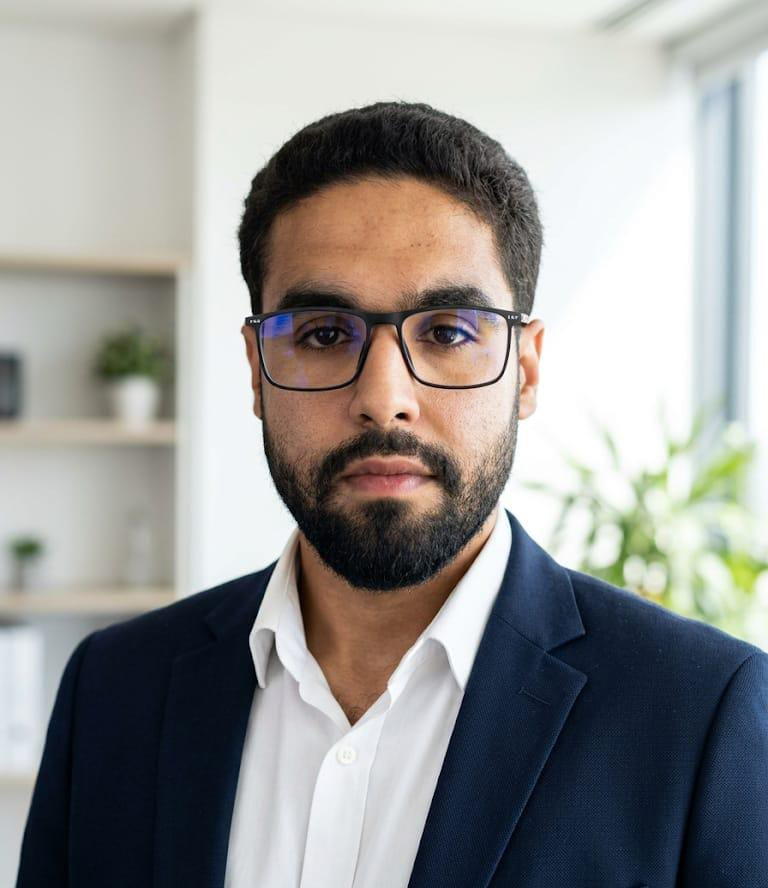
\includegraphics[width=1.70cm,height=1.70cm]{../master_ssot/hamza.jpeg}};
    \end{tikzpicture}
\end{minipage}

\vspace{0.3cm}

% --- PROFIL ---
\section*{PROFIL}
\noindent Étudiant en Infrastructures Digitales avec une spécialisation forte en Opérations de Sécurité (SecOps) et Blue Teaming. Profil orienté vers l'audit, le durcissement d'endpoints (Zero-Trust), et la télémétrie SIEM (Wazuh). Capacité démontrée à sécuriser des infrastructures réseau sur site sous contraintes strictes (marchés publics) et à intégrer l'automatisation pour la défense des systèmes (IaC). 

% --- COMPÉTENCES TECHNIQUES ---
\section*{COMPÉTENCES TECHNIQUES}
\begin{itemize}[leftmargin=*, itemsep=0.0pt, parsep=0pt, topsep=0pt]
    \item \textbf{Blue Teaming \& SIEM :} Architecture et déploiement Wazuh (FIM, IDS), Supervision réseau (Zabbix), Audit de sécurité, Détection d'anomalies, Analyse de vulnérabilités.
    \item \textbf{Sécurité Endpoint \& Identité :} Durcissement de systèmes (Linux/Windows), Zero-Trust (Anti-BadUSB, restriction des montages), AD DS, Contrôle d'accès centralisé (RADIUS/NPS).
    \item \textbf{Sécurité Réseau (L2/L3) :} Sécurisation Cisco IOS / Ruijie, Isolation par VLAN, Filtrage de trafic, Adressage IPv4/IPv6 sécurisé, Sécurité CCTV (NVR Hikvision).
    \item \textbf{Automatisation de Défense :} Scripts de remédiation (Bash, PowerShell, Python), Infrastructure as Code (Ansible, YAML), Intégration API.
    \item \textbf{Environnements :} EVE-NG, GNS3, VMware Workstation, Proxmox, Git/GitHub.
\end{itemize}

% --- EXPÉRIENCE PROFESSIONNELLE ---
\section*{EXPÉRIENCE PROFESSIONNELLE}
\noindent
\textbf{Technicien Sécurité \& Réseaux} \hfill \textit{Avril -- Juin 2026}\\
\textit{24CONFIG Technology -- Marrakech}
\begin{itemize}[leftmargin=*, itemsep=0.0pt, parsep=0pt, topsep=0pt]
    \item \textbf{Sécurité des Marchés Publics :} Intégration logique et sécurisation d'infrastructures réseaux critiques (Milieu de la Justice et Pénitentiaire).
    \item \textbf{Contrôle d'Accès :} Configuration de serveurs RADIUS (NPS Windows Server) pour garantir un accès réseau centralisé et authentifié.
    \item \textbf{Conformité \& Audit :} Recette de conformité de la couche physique et tests pour éliminer les vulnérabilités liées à l'atténuation du signal.
    \item \textbf{Ségrégation Réseau :} Isolation des réseaux IP CCTV sur des commutateurs multi-vendeurs pour prévenir les accès non autorisés.
\end{itemize}

\vspace{-0.15cm}
\noindent
\textbf{Technicien Déploiement Sécurisé} \hfill \textit{Juillet -- Août 2025}\\
\textit{ISGI Azli -- Marrakech}
\begin{itemize}[leftmargin=*, itemsep=0.0pt, parsep=0pt, topsep=0pt]
    \item \textbf{Durcissement Système :} Conception d'une image système Windows Master (Golden Image) intégrant les politiques de sécurité de base.
    \item \textbf{Provisioning Automatisé :} Déploiement sécurisé de masse via WDS sur l'ensemble du parc informatique pour garantir l'uniformité de la surface d'attaque.
\end{itemize}

% --- PROJETS TECHNIQUES & R&D ---
\section*{PROJETS TECHNIQUES \& R\&D}
\noindent
\textbf{Hub Centralisé d'Observabilité et de Sécurité (SIEM \& Zero-Trust)}\\
Déploiement d'une architecture de supervision combinant Zabbix et Wazuh SIEM. Durcissement d'hôtes Linux par politiques strictes orientées Zero-Trust pour bloquer le montage automatique et isoler les périphériques de blocs (prévention des attaques BadUSB et exfiltration).
\textbf{Orchestration \& Déploiement Automatisé de Sécurité (Ansible / Python / Nmap)}\\
Conception d'un système de provisionnement de sécurité à l'échelle de l'entreprise. Scripting Python couplé à Nmap pour scanner le réseau et profiler les cibles. Exécution conditionnelle de playbooks Ansible poussant massivement les agents SIEM (Wazuh) et de télémétrie (Zabbix) sur les endpoints (Linux/Windows) via SSH/WinRM pour une couverture de surveillance totale.
\textbf{Automatisation Sécurisée Multi-vendeurs (IaC / Ansible / Python)}\\
Développement de playbooks Ansible basés sur un modèle SSOT (Single Source of Truth) pour déployer des configurations réseau standardisées et sécurisées sur Cisco et Ruijie, minimisant les erreurs manuelles de configuration (misconfigurations).

% --- CERTIFICATIONS ---
\section*{CERTIFICATIONS}
\begin{itemize}[leftmargin=*, itemsep=0.0pt, parsep=0pt, topsep=0pt]
    \item \textbf{Cybersécurité (En cours - 2026) :} Cisco CyberOps Associate \textbar{} Cisco DevNet Associate.
    \item \textbf{Certificats Validés :} Introduction à la Cybersécurité \textbar{} CCNA Academy (ITN \textbar{} SRWE \textbar{} ENSA) \textbar{} Python Essentials 1 \& 2 \textbar{} Linux Essentials \& Linux 2 \textbar{} IT Essentials.
\end{itemize}

% --- FORMATION ---
\section*{FORMATION}
\noindent \textbf{Technicien Spécialisé : Infrastructures Digitales (Systèmes \& Réseaux)} \hfill \textit{ISGI Marrakech -- 2024--2026}\\
\noindent \textbf{Faculté des Sciences Semlalia -- Univ. Cadi Ayyad (Sciences Maths Appliquées)} \hfill \textit{2022--2024}\\
\noindent \textbf{Classes Préparatoires (ECS)} \hfill \textit{Lycée Reda Slaoui Agadir -- 2020--2022}\\
\noindent \textbf{Baccalauréat : Sciences Mathématiques} \hfill \textit{Lycée Mohamed VI Marrakech -- 2019--2020}

% --- LANGUES ---
\section*{LANGUES}
\noindent \textbf{Arabe :} Maternelle \quad \textbar{} \quad \textbf{Français :} C1 (Professionnel) \quad \textbar{} \quad \textbf{Anglais :} C1 (Technique avancé)

\end{document}
